\documentclass{article}

% 33.1 inches by 46.8 inches
% 841 mm by 1189 mm
\usepackage[a2paper, margin=.3in, top=1in]{geometry}

% Grid size of 1.48 inches
% Need: 16x31 grid.
% 23 in by 45.88 in

% margin of .3 inches keeps us within bounds.

\usepackage{tikz}

\setlength{\parindent}{0pt}

\begin{document}
\begin{center}
\noindent
\scalebox{3}{\Huge Cellular Automaton : Rule 90}\\[.8in]
%\scalebox{2}{\begin{minipage}{3in}\Huge Repeatedly apply these\\
%             rules downward.\end{minipage}}\\[.5in]
\begin{minipage}{.25\linewidth}
\begin{center}
{\Huge
The color of each hexagon is determined by the colors of the hexagons above it.
}\\[.5in]
\begin{tikzpicture}
  \node at (0,0) {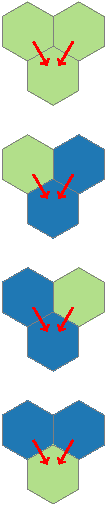
\includegraphics[scale=3]{rule90_hexrules_vertical_arrows.pdf}};
\end{tikzpicture}\\[.5in]
{\Huge Repeatedly apply these rules down the lattice.}
\end{center}
\end{minipage}\hspace{.7in}
\begin{minipage}{.7\linewidth}
\scalebox{2}{\Huge Before}\\[.5in]
\begin{tikzpicture}
  \node at (0,0) {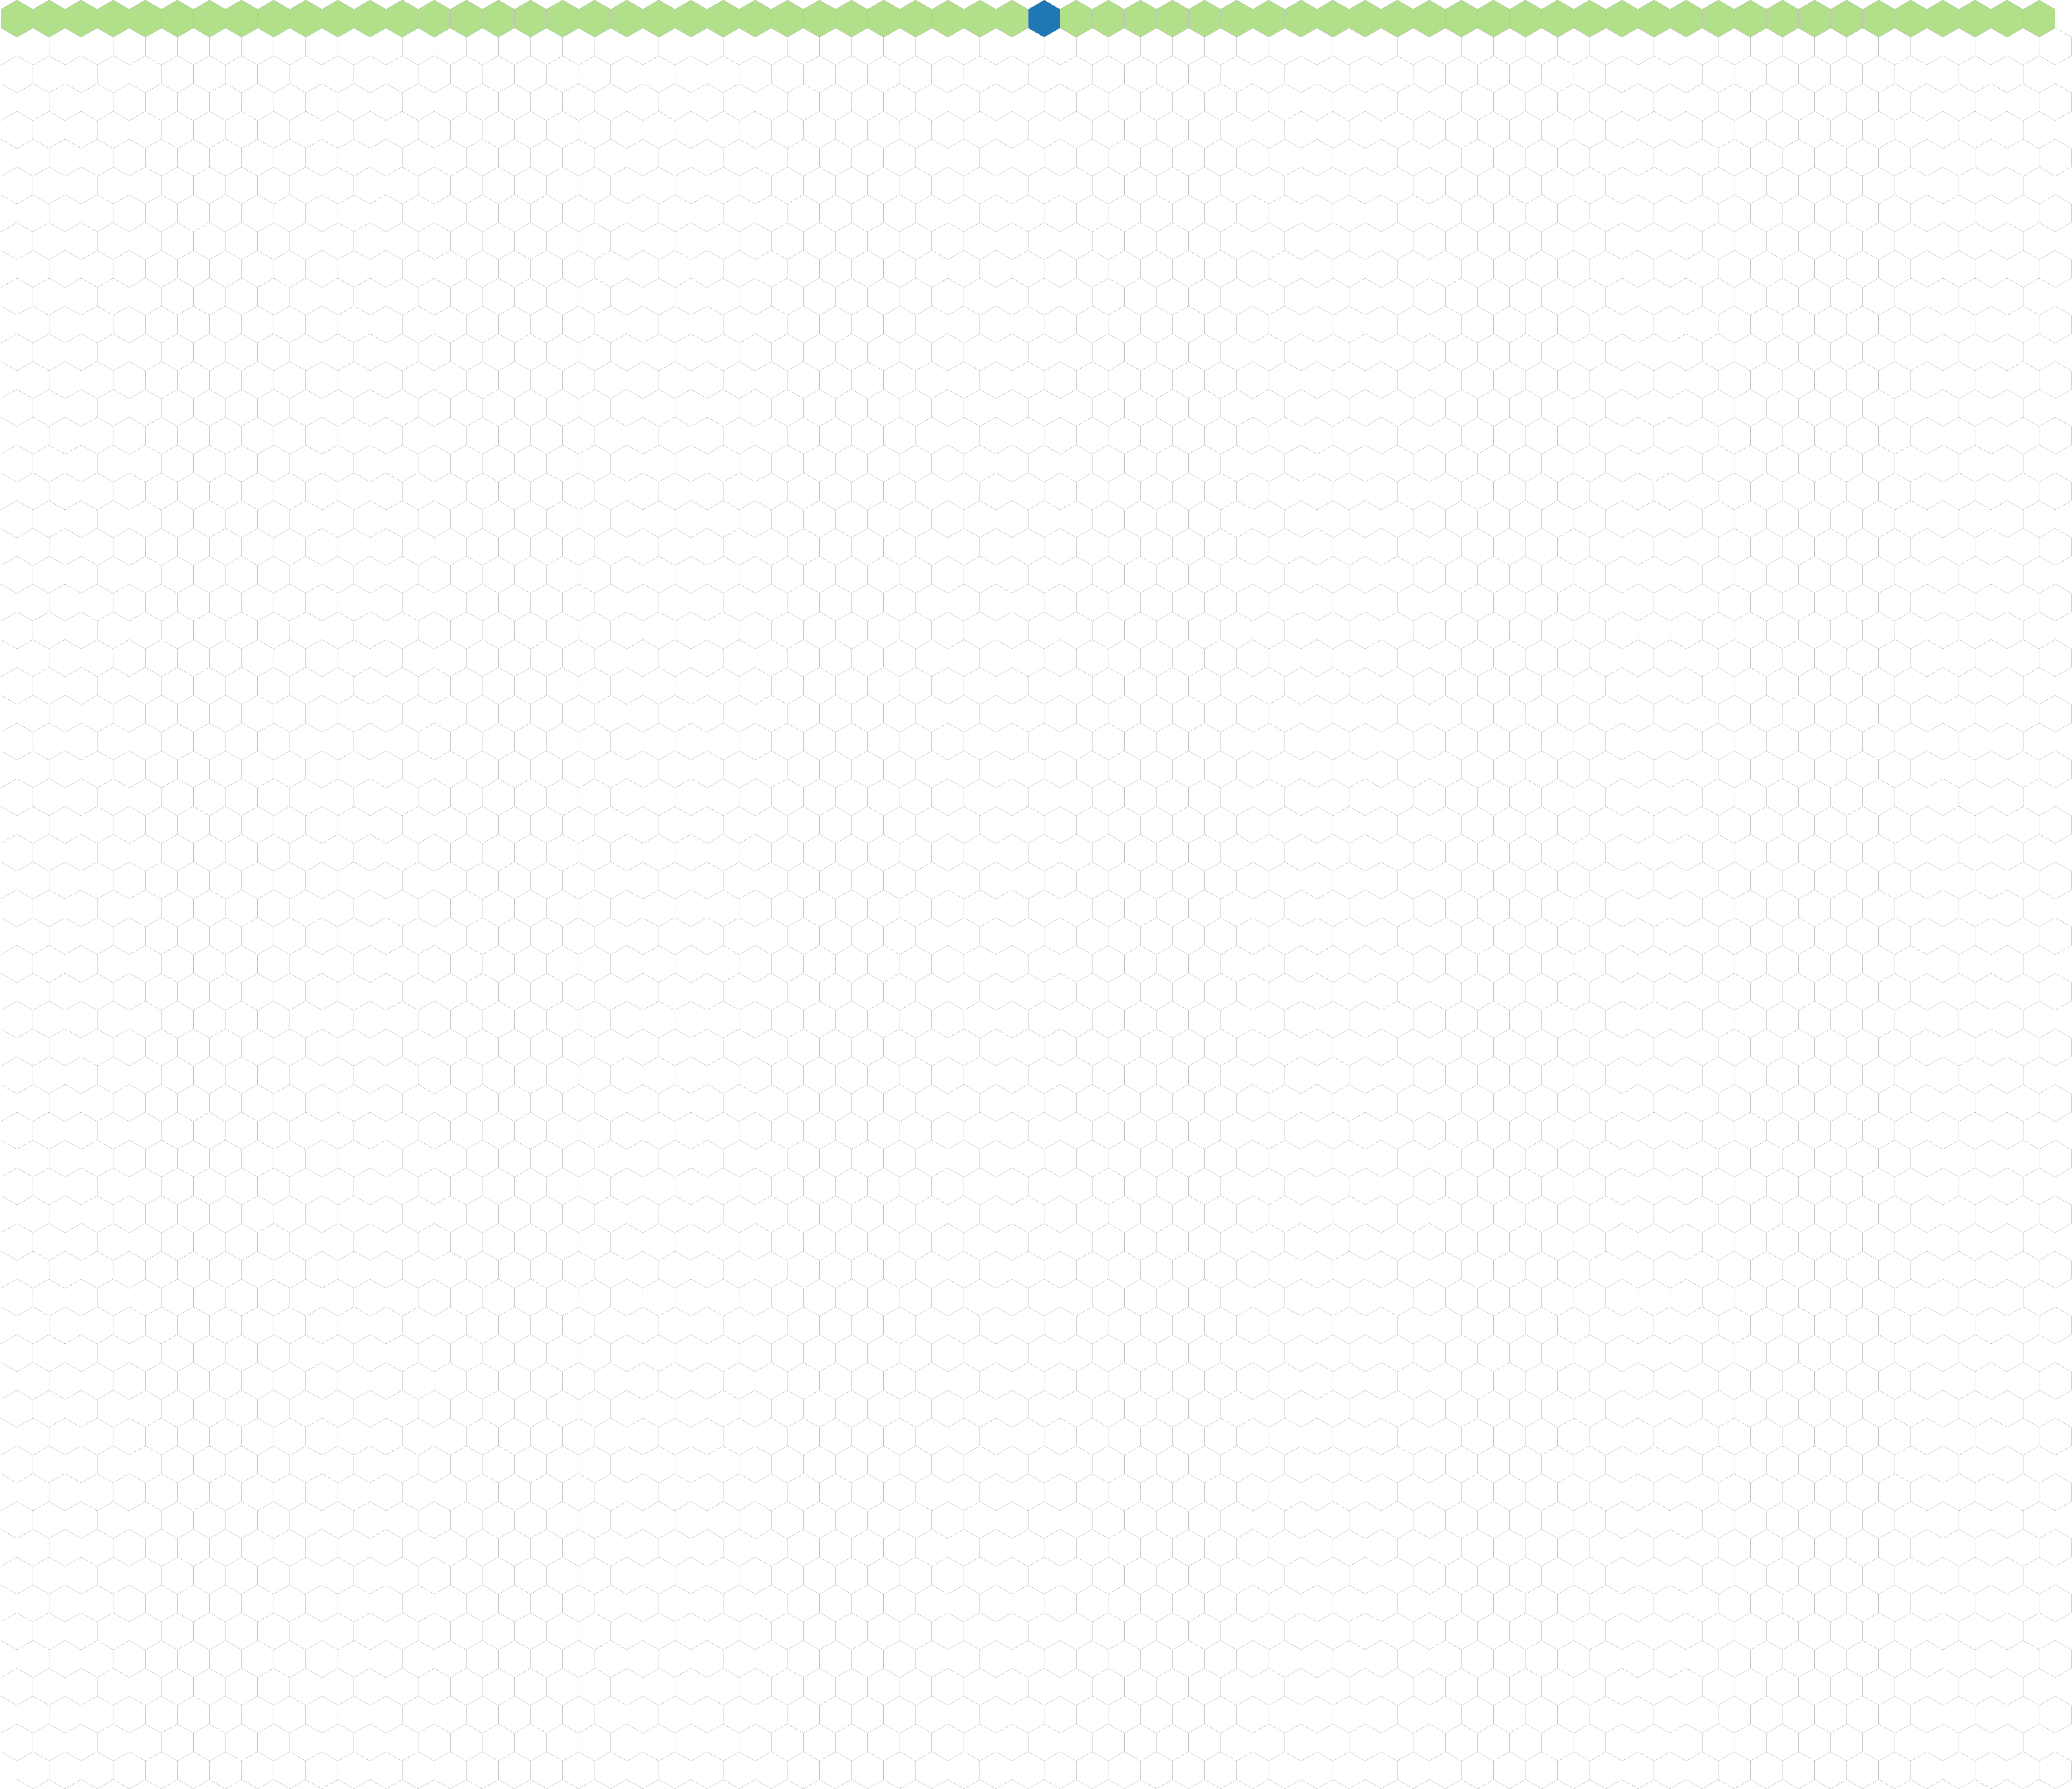
\includegraphics[scale=.3]{hexlattice_1.pdf}};
\end{tikzpicture}\\[1in]
\scalebox{2}{\Huge After}\\[.5in]
\begin{tikzpicture}
  \node at (0,0) {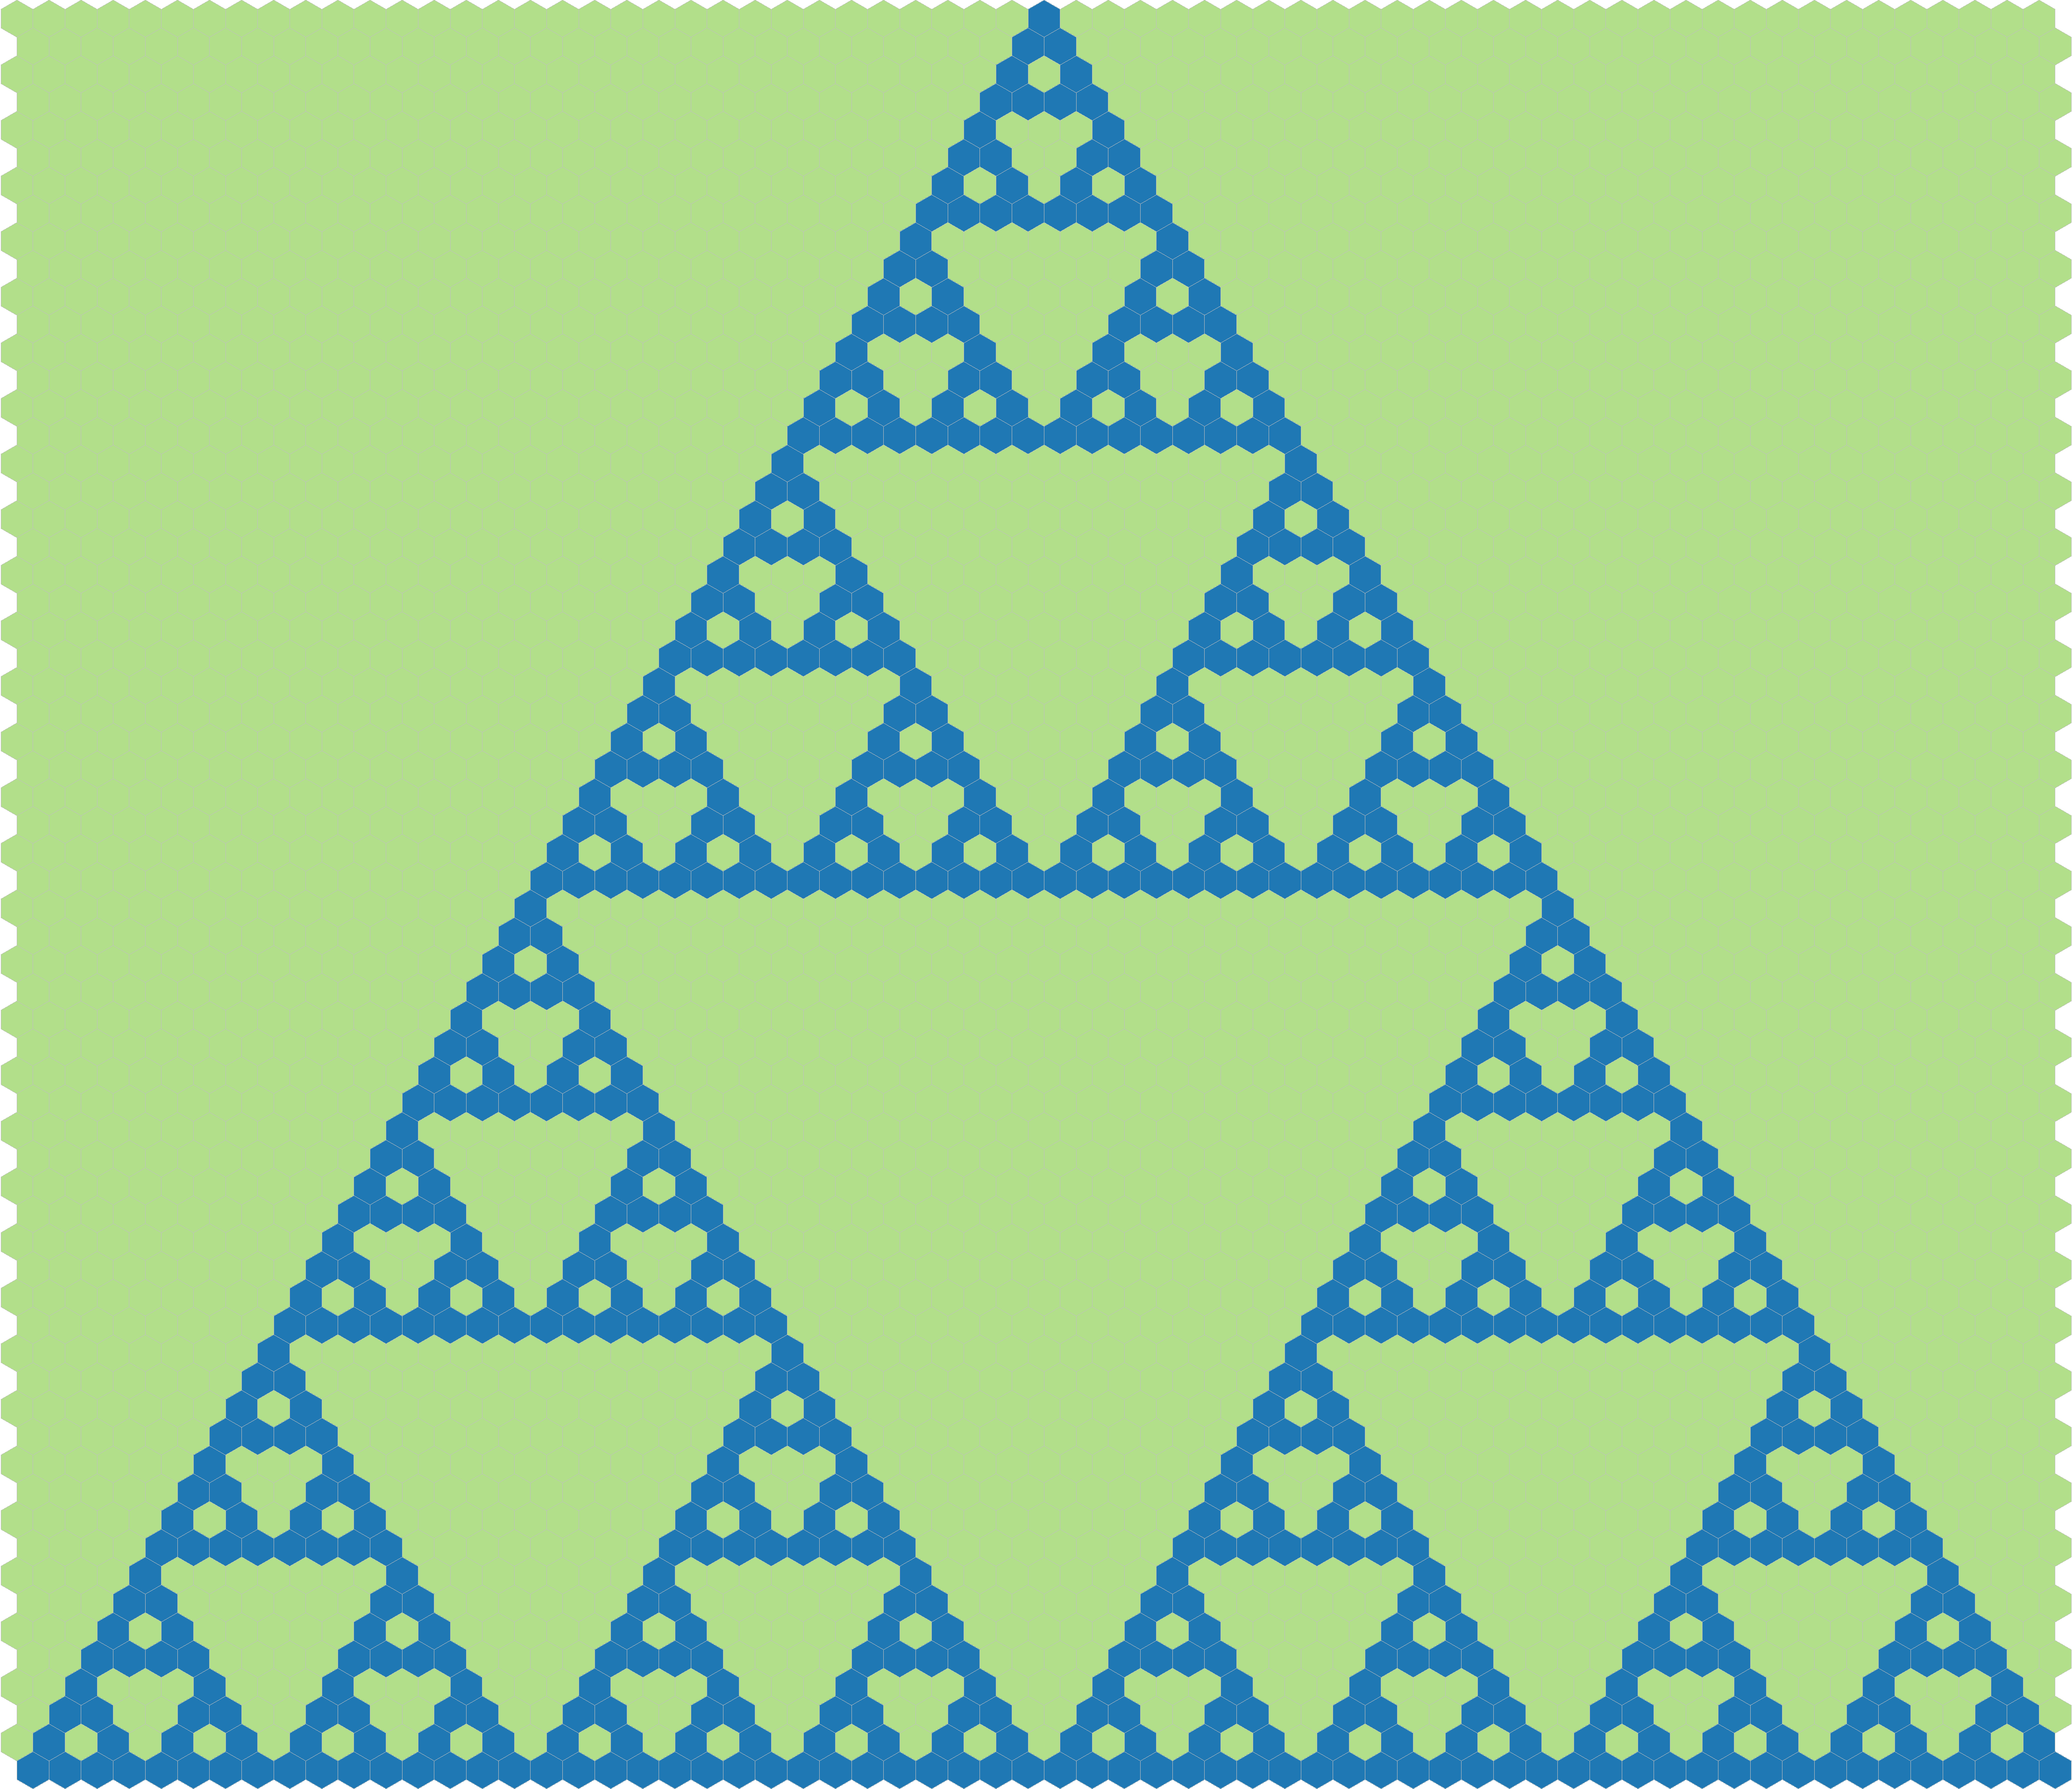
\includegraphics[scale=.3]{hexlattice_2.pdf}};
\end{tikzpicture}
\end{minipage}
\end{center}
\end{document}

